\chapter[Lemmas concerning minimum modulus of...]{Lemmas concerning minimum modulus of canonical products}\label{chap14} %lecte14

We\pageoriginale need certain lemmas to find minorization of $\big| C (w)\big|$

\begin{lem}\label{chap14:lem1} %lem 1
 Suppose $\bar{D}^. < \infty$. Let $C (w) = \prod \left(1 - \dfrac {w^2}
 {\lambda^2}\right)$. Given $\varepsilon > 0$, there exists an infinity of
 $R_j \nearrow \infty$ such that for $|w| =R_j$ we have $\big| C
 (w) \big| > e^{- \varepsilon R_j}$. 
\end{lem}

\begin{proof}
 We have $\bigg| C (w)\bigg| \ge \bigg| 1 - \dfrac
 {r^2}{|\lambda^2|}\bigg|$, where $|w| = r$. We apply Carleman's
 formula to the function $C^* (w) = \prod \left(1 - \dfrac {w^2}
 {|\lambda^2|}\right)$, in the upper half plane $v \ge 0$. Then we have
 the following relation: 
 \begin{equation}
 \int^R_{-R} \log \big| C^* (u) \big| \frac{du} {u^2} = o
 \tag{1}\label{chap14:eq1} 
 \end{equation}
 This relation implies that there exists an infinity of $R_j \nearrow
 \infty$ such that $\log \big| C^* (R_j)\big| > - \varepsilon R_j ;
 i.e \text{ for } |w| = R_j |C (w) | \ge |C^* (R_j)| > e^{-
 \varepsilon R_j}$. 
\end{proof}

\begin{lem}[H. Cartan]\label{chap14:lem2}
 Suppose $\delta > 0$ and $M_1, \ldots,M_n$ are $n$
 given points in the complex plane. Then we can find $m$ discs, $m
 \le n$ the sum of whose radii is $2n \delta$ in such a manner that
 if $M$ is any point outside these discs the product of the
 distances $MM_1, \ldots, MM_n > \left(\dfrac {n \delta} {e}\right)^n$. 
\end{lem}

\begin{proof}
 Let $k_1$ be the largest integer such that there exists a disc of
 radius $k_1 \delta$ containing at least $k_1$ of the points $M_j$,
 and let $C_1$ be such a disc. Obviously $C_1$ contains exactly $k_1$
 points $M_j$. Let us remove these $k_1$ points, and define in the
 same manner from the remaining points (if there exist any ) a disc $C_2$
 of radius $k^\delta_2$, and so on: we get a finite number of discs,
 say $C_1, \ldots,C_m$, of radii $k_1 \delta, \ldots,k_m \delta$,\pageoriginale and
 $k_1 +\cdots+ k_m=n$. Now, let $\Gamma_1, \ldots, \Gamma_m$ be discs
 concentric with $C_1\ldots C_m$ and of twice the radii. From the 
 construction of $C_1, \ldots,C_m$, it follows that, if a disc $\int
 (M, k \delta)$ of center $M$ and radius $k \delta$ contains at
 least $k$ points $M_j$, then it contains a point $M_q \in
 C_q$ with $k_q \ge k$; thus $M \in \Gamma_q$. 
\end{proof}

Suppose now $M \notin \cup \Gamma_j$; then, ever $\int (M, k \delta)$
contains at most $k-1$ points $M_j$. Let the distances $MM_j$ be that
$MM_1 \le MM_2 \cdots MM_n$. Then $MM_1 > \delta, MM_2 > 2 \delta
,\ldots, MM_n > n \delta$, and 
$$
MM_1 \cdot MM_2 \cdots MM_n > n! \delta^n > \left(\frac{n \delta}{e}\right)^n
$$
that completes the proof.

\noindent \textbf{Definitions. }
 Given a finite set of points $\{ M_j\}$ and $ \delta > 0$, we call
 $\{ \Gamma_j\}$ a system of ``Cartan discs relative to $\{ M_j\}$
 and $\delta$''. 

Let $\Lambda$ be a sequence of points in the complex plane without
finite points of accumulation, and $\delta > 0$. By a system of
``Cartan discs relative to $\Lambda$ and $\delta$'', we shall mean the
union of the system of Cartan discs relative to $\Lambda$ and the
annulus $2^n - 1 \le |z| < 2^{n+1} - 1 (n = 0, 1,\ldots,)$ 

\begin{lem}\label{chap14:lem3}
  Suppose the symmetrical sequence $\Lambda$ has a density $D$. Given
  $\varepsilon > 0$ and $\delta > 0$ we have $|C (w)| = \prod | 1-w^2
  / \lambda^2 | > e^{- \varepsilon}|w|$ for $|w|$ sufficiently large,
  and $w$ varying outside Cartan discs of a system relative to
  $\Lambda$ and $\delta$. 
\end{lem}

\begin{proof}
  Write $C (w) = \prod\limits_1 \prod\limits_2 \text { where }
  \prod\limits_1 = \prod\limits_{r / \gamma < |\lambda| < \gamma_r}
  (1-w^2 / \lambda^2), \gamma > 1$ to be chosen later to be near
  $1$. Denoting by $n (r)$ the distribution function of $\{
  |\lambda|\}$, we have the following relations: 
  \begin{align*}
 \log |\prod_2| & >\left\{ \int\limits^{r/ \gamma}_o + \int^{\infty}_{r
 \gamma}\right\} \left[ \log \big| 1- \frac{r^2} {\lambda^2}\big| dn
 (\lambda)\right] (r = |w|)\\ 
 & = n \left(\frac{r}{\gamma}\right) \log (\gamma^2-1) - n (\gamma
 r) \log \left(1 - \frac{1}{\gamma 2}\right)\\ 
 &\quad + r \int^{1/\gamma}_0 \frac{2}{1-u^2} D (ru) du -
 \int^\infty_\gamma \frac{2}{u^2 -1} D (ru) du 
 \end{align*}
 $$
 \displaylines{\hfill 
 \int\limits^{1/\gamma}_o \frac{2}{u^2-1} D(ru) du < \log \frac{ \gamma +
  1}{\gamma - 1} (D + 0(1)) \quad (r \to \infty)\hfill \cr 
 \text{and}\hfill \int^\infty_\gamma \frac{2}{u^2-1} D(ru) du < \log \frac{
  \gamma + 1}{\gamma - 1} (D + 0(1)) \quad (r \to \infty) \hfill \cr
 \hfill n \left(\frac{r}{\gamma}\right) \log (\gamma^2 -1) - n (\gamma r) \log \left(1 -
 \frac{1}{\gamma^2}\right) > 2 \log \gamma . n (\gamma r) > 0\hfill } 
 $$
if\pageoriginale $\gamma^2 < 2$. Then $\log \big| \prod_2\big| > - \varepsilon/2$
 if $\gamma^2 < 2$, and $r$ large enough. Now $\prod_1$ is a product
 of $N$ terms, $N < 2D_r (\gamma - 1 /\gamma)$, if $r$ is large
 enough. Let $\prod_{1,n}$ be the product of those terms, whose zeros
 are in use in the annulus $2^n- 1 \le |z| \le 2^{n+1} -1; \prod_1 $
 can be written as $\prod_{1,n}. \prod_{1,n+1}$ for a convenient
 $n$. Take $w$ outside any Cartan disc and suppose (if necessary, by
 changing the sign of $\lambda$) $|w -\lambda| \le |w+\lambda|$;
 then 
 $$
 \big| \prod_{1,n}\big| > \prod_{1,n}\big| 1 -\frac{w}{\lambda}\big| 
 > \frac{1}{(\gamma r)^M} \prod_{1,n} \big| w-\lambda \big| > 
 \frac{1}{(\gamma r)^M} \left(\frac{M\delta}{e}\right)M 
 $$
 where $M$ is the number of terms of $\prod_{1,n}; M \le N < 2D r
 (\gamma - \dfrac{1}{\gamma})$ 
 $$
 \log \big| \prod_{1,n}\big| > M \log \frac{m}{\gamma er} = r 
 \frac{M}{r} \left(\frac{M}{r}. \frac{\delta}{\gamma^e}\right) > -
 \frac{\varepsilon}{4} r, 
 $$
 if $\gamma$ is chosen near enough to $1$. That completes the proof.
\end{proof}

\begin{lem}\label{chap14:lem4}
 Suppose $\sum \dfrac{1}{\lambda} < \infty$ and $ C(w) = \prod ( 1
 -\dfrac{w^2}{\lambda^2})$. For almost all $\theta$, we have
 $\lim\limits_{r \to \infty} \log \dfrac{|C (r e^{i \theta})|} {r} =
 0$. 
\end{lem}

\begin{proof}
 We choose the set of `` Cartan discs", $\Gamma$, as in the previous
 lemma. Let $\theta_\Gamma$ be the angle which a circle $\Gamma$
 subtends at origin. Since the radius of the circle $\Gamma$ are of
 the from $2 n \delta$ with precisely $n$ points $\lambda$ in side
 $\Gamma$, we have $\theta_\Gamma \sim \sum\limits_{\lambda
 \in \Gamma} \dfrac{1}{|\lambda|}$ and $ \sum
 |\theta_\Gamma| < \infty$ 
\end{proof}

\begin{figure}[H]
\centerline{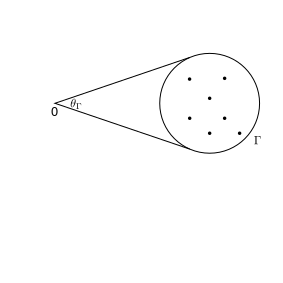
\includegraphics{vol15-figures/fig15-11.eps}}
\end{figure}

If\pageoriginale we consider only those circles far away from the origin, we have
$\sum |\theta_\Gamma| < \varepsilon$. Then outside of these angles
$\theta $, by the previous lemma, we have $|C (w)| > e^{-
 \varepsilon} |w|$. Thus we have $\lim \dfrac{\log |C (w)|} {r}$=0
almost everywhere. 

One can prove, in the same manner, the following lemma. 

\begin{lem}\label{chap14:lem5}
 If $D = 0$, then $\lim \dfrac{\log |C (w)|} {r} = 0$, when $ w \to
 \infty$, $w$ vary ing outside of Cartan discs associated with
 $\Lambda$. 
\end{lem}

\begin{lem}\label{chap14:lem6}
 Let $\Phi (w)$ and $\psi (w)$ be two functions of exponential
 type. Suppose $|\Phi (w)| < |\psi (w)| < e^{|v|}$ outside of discs
 $\Gamma$, each of which is of radius $2 k \varepsilon (k = k (\Gamma)$:
 an integer) and contains $k$ zeros of $\psi$. Then, for sufficiently
 small $\varepsilon, |\Phi (w)| < e^{|v|}$. 
\end{lem}

\begin{proof}
 Let $w$ belong to the frontier of a $\Gamma$. Applying Jensen's
 formula to $\psi$ on a circle $C$ of center $w$ and radius $r$, we
 get 
 \begin{gather*}
 \log |\psi (w)| < \frac{1}{2 \pi} \int^{2 \pi}_0 \log |\psi (w) +
 re^{i \theta} | d \theta- \log \frac{r^k}{(2 k \varepsilon)^k}\\ 
 < |v| + \frac{2}{\pi}r - r \frac{k}{r} \log \frac{r}{ 2 k
  \varepsilon} < |v| -r 
 \end{gather*}
 for $r = k$ and $\varepsilon$ small. Applying Cauchy's theorem for
 $\Phi (w)$ on $C$, 
 \begin{figure}[H]
 \centerline{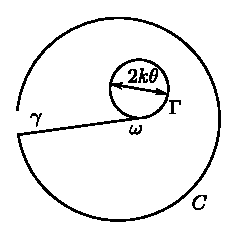
\includegraphics{vol15-figures/fig15-12.eps}}
 \end{figure}
 $$
 |\Phi (w)| < e^{\max |v| -r} ~\text{ for }~ w' \in C. ~\text{
 So }~ |\Phi (w)| < c^{|v|} 
 $$ 
\end{proof}

\begin{lem}\label{chap14:lem7}
 If $\Lambda$ has a density $D$ and if arg $\lambda \to 0$, then
 $\lim \frac{\log |C(w)|} {r} = \pi D |\sin \theta| \text{ for }
 \theta \nequiv 0 (\mod \pi) $. (Cf. Method of Carlson, lecture $10 \S 1$) 
\end{lem}

\begin{lem}\label{chap14:lem8}
  If $\lambda_n$ are real, $|C (re^{i \theta})| > 1 \text{ if }
  |\theta \pm \frac{\pi}{2}| < \frac{\pi}{4}$. The proof is obvious. 
\end{lem}
